\documentclass[tikz, border=10pt]{standalone}

\usetikzlibrary{arrows}

\begin{document}
	
	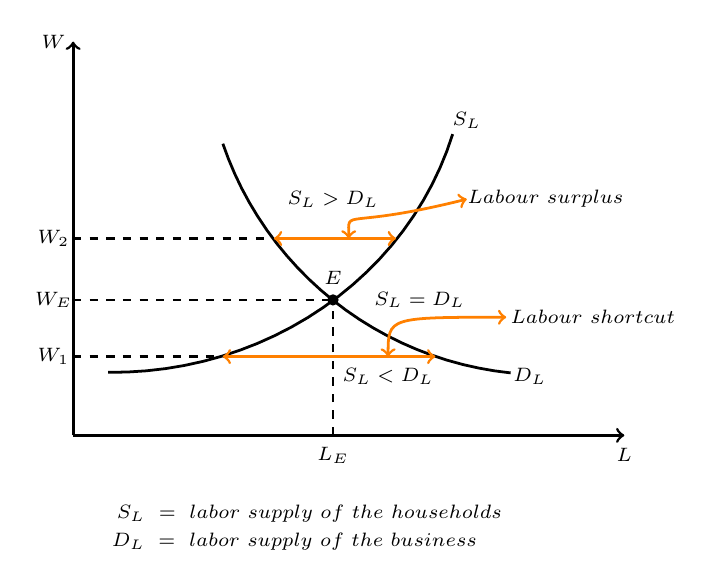
\begin{tikzpicture}[line width=1pt]
		\draw[->] (0, 0) -- (7, 0);
		\draw[->] (0, 0) -- (0, 5);
	
		\draw [shift={(0.5, 5)}] plot[domain=4.7:6,variable=\t]({1*4.5*cos(\t r)+-0*4.2*sin(\t r)},{0*3.8*cos(\t r)+1*4.2*sin(\t r)});
		\draw [shift={(6, 5.1)}] plot[domain=3.47:4.61,variable=\t]({1*4.33*cos(\t r)+-0*4.33*sin(\t r)},{0*4.33*cos(\t r)+1*4.33*sin(\t r)});
		
		\draw [dashed] (0, 1.72) -- (3.3, 1.72);
		\draw [dashed] (3.3, 0) -- (3.3, 1.72);
		
		\draw [dashed] (0, 2.5) -- (2.5, 2.5);
		\draw [dashed] (0, 1) -- (1.9, 1);
		
		\draw[<->, color=orange] (1.9, 1) -- (4.6, 1);
		\draw[<->, color=orange] (2.55, 2.5) -- (4.1, 2.5);
		
		\draw[<->, color=orange] (3.5, 2.5) .. controls (3.5, 2.9) and (3.4, 2.6) .. (5, 3);
		\draw[<->, color=orange] (4, 1) .. controls (4, 1.5) and (4, 1.5) .. (5.5, 1.5);
	\begin{scriptsize}
	
		\draw (3.3, 2) node {$E$};
	
		\draw (-0.25, 2.5) node {$W_2$};
		\draw (-0.25, 1.72) node {$W_E$};
		\draw (-0.25, 1) node {$W_1$};
		\draw (3.3, -0.25) node {$L_E$};
		
		\draw (-0.25, 5) node {$W$};
		\draw (7, -0.25) node {$L$};
		
		\draw (5, 4) node {$S_L$};
		\draw (5.8, 0.75) node {$D_L$};
		
		\draw (3.3, 3) node {$S_L > D_L$};
		\draw (4.4, 1.72) node {$S_L = D_L$};
		\draw (4, 0.75) node {$S_L < D_L$};
		
		\draw (6, 3) node {$Labour~surplus$};
		\draw (6.6, 1.5) node {$Labour~shortcut$};
		
		\draw (3, -1) node {$S_L~=~labor~supply~of~the~households$};
		\draw (3, -1.35) node {$D_L~=~labor~supply~of~the~business~~~~$};
		
		\draw[fill=black] (3.3, 1.72) circle (1.5pt);
		\end{scriptsize}
\end{tikzpicture}
\end{document}